To test these three algorithms, we ran two simulation studies in which we simulated a total of $T = 10^{5}$ observations from an HMM with $N = 3$ hidden states. For both simulation studies, we used the same distribution for $Y | X = i$ for $i = 1,2,3$. In particular, $Y_t | X_t = i$ follows a normal distribution with mean $\mu^{(i)}$, and standard deviation $\sigma^{(i)}$, where
%
\begin{equation*}
    \mu^{(1)} = 0, \quad \sigma^{(1)} = e^{-1}, \qquad
    \mu^{(2)} = 1, \quad \sigma^{(2)} = e^{1}, \qquad
    \mu^{(3)} = 2, \quad \sigma^{(3)} = e^{0}.
\end{equation*}
%
The transition probability matrices changed between the two experiments (see the subsequent subsections for details).

We initialized $\eta[0]$ for all algorithms such that the transition probability matrix $\Gamma[0]$ was equal to the true $\Gamma$ associated with the data generation process. We initialized the parameters $\theta[0]$ as follows:
%
\begin{equation*}
    \mu^{(1)}[0] = -1.0, \quad \sigma^{(1)}[0] = e^{0}, \qquad
    \mu^{(2)}[0] = 1.1, \quad \sigma^{(2)}[0] = e^{0}, \qquad
    \mu^{(3)}[0] = 2.1, \quad \sigma^{(3)}[0] = e^{0}.
\end{equation*}
%
We set the step size to be $\lambda^\theta = \lambda^\eta = 0.01$. 

If the 2-norm of the average estimated gradient $||\frac{1}{T}\sum_{t=1}^T \widehat \nabla F^{(k,m)}_t + \widehat \nabla G^{(k,m)}_t||$ ever fell below a tolerance of $10^{-8}$, we terminated the M-step of algorithm and moved on to the E-step. Likewise, if the relative change of the log-likelihood after one full E- and M- step of the EM algorithm ever fell below a tolerance of $10^{-10}$, we terminated the algorithm altogether. We found the ground truth MLEs by running the traditional EM algorithm until the relative change in the log-likelihood was on the order of machine precision $10^{-15}$.

\subsection{Experiment one: slow mixing}

The first experiment was to test the performance of the algorithm for a rapidly mixing HMM. As such, we used the following transition probabilities:
%
\begin{equation*}
    \Gamma = 
    \begin{pmatrix} 
        0.9 & 0.05 & 0.05 \\
        0.05 & 0.9 & 0.05 \\
        0.05 & 0.05 & 0.9
    \end{pmatrix},
    \qquad
    \delta = \begin{pmatrix} 0.33 & 0.33 & 0.33 \end{pmatrix}.
\end{equation*}
%
Figure (\ref{fig:exp1_ll}) displays the log-likelihood of the MLE parameters minus the log-likelihood at each epoch. 

SAGA without a partial E-step performs similarly to the EM algorithm in a per-epoch basis because SAGA is successfully converging for the M-step when $M = T$. However, it does not perform as well as the EM algorithm on a per-time basis because the M-step is significantly slower when using SAGA vs the closed-form solution. This behaviour is expected, and SAGA has a significant advantage over the EM algorithm in that it only requires gradients rather than sufficient statistics.

Implementing a partial E-step shows that SAGA can outperform the EM algorithm when the parameter estimates are far from the optimal solutions and when the underlying HMM does not mix rapidly. This is likely because the weights of the $F$ and $G$ are very inaccurate at first, and updating them early in the optimization procedure yields a significant speed-up. In addition, if the Markov chain is rapidly mixing, then updates to $\gamma_{t_m}$ and $\xi_{t_m}$ at a single data point are more accurate. Future work may involve performing the partial-E step for many weights at once sequentially, depending upon the mixing time of the current estimate of $\eta[k]$.

\begin{figure}
    \centering
    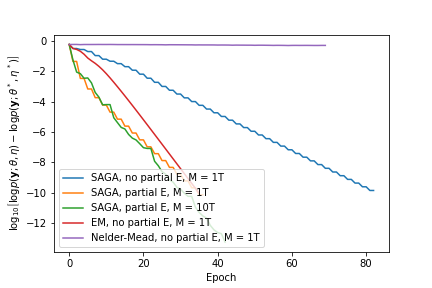
\includegraphics[width=3in]{../plt/log-like_v_epoch_exp_1.png}
    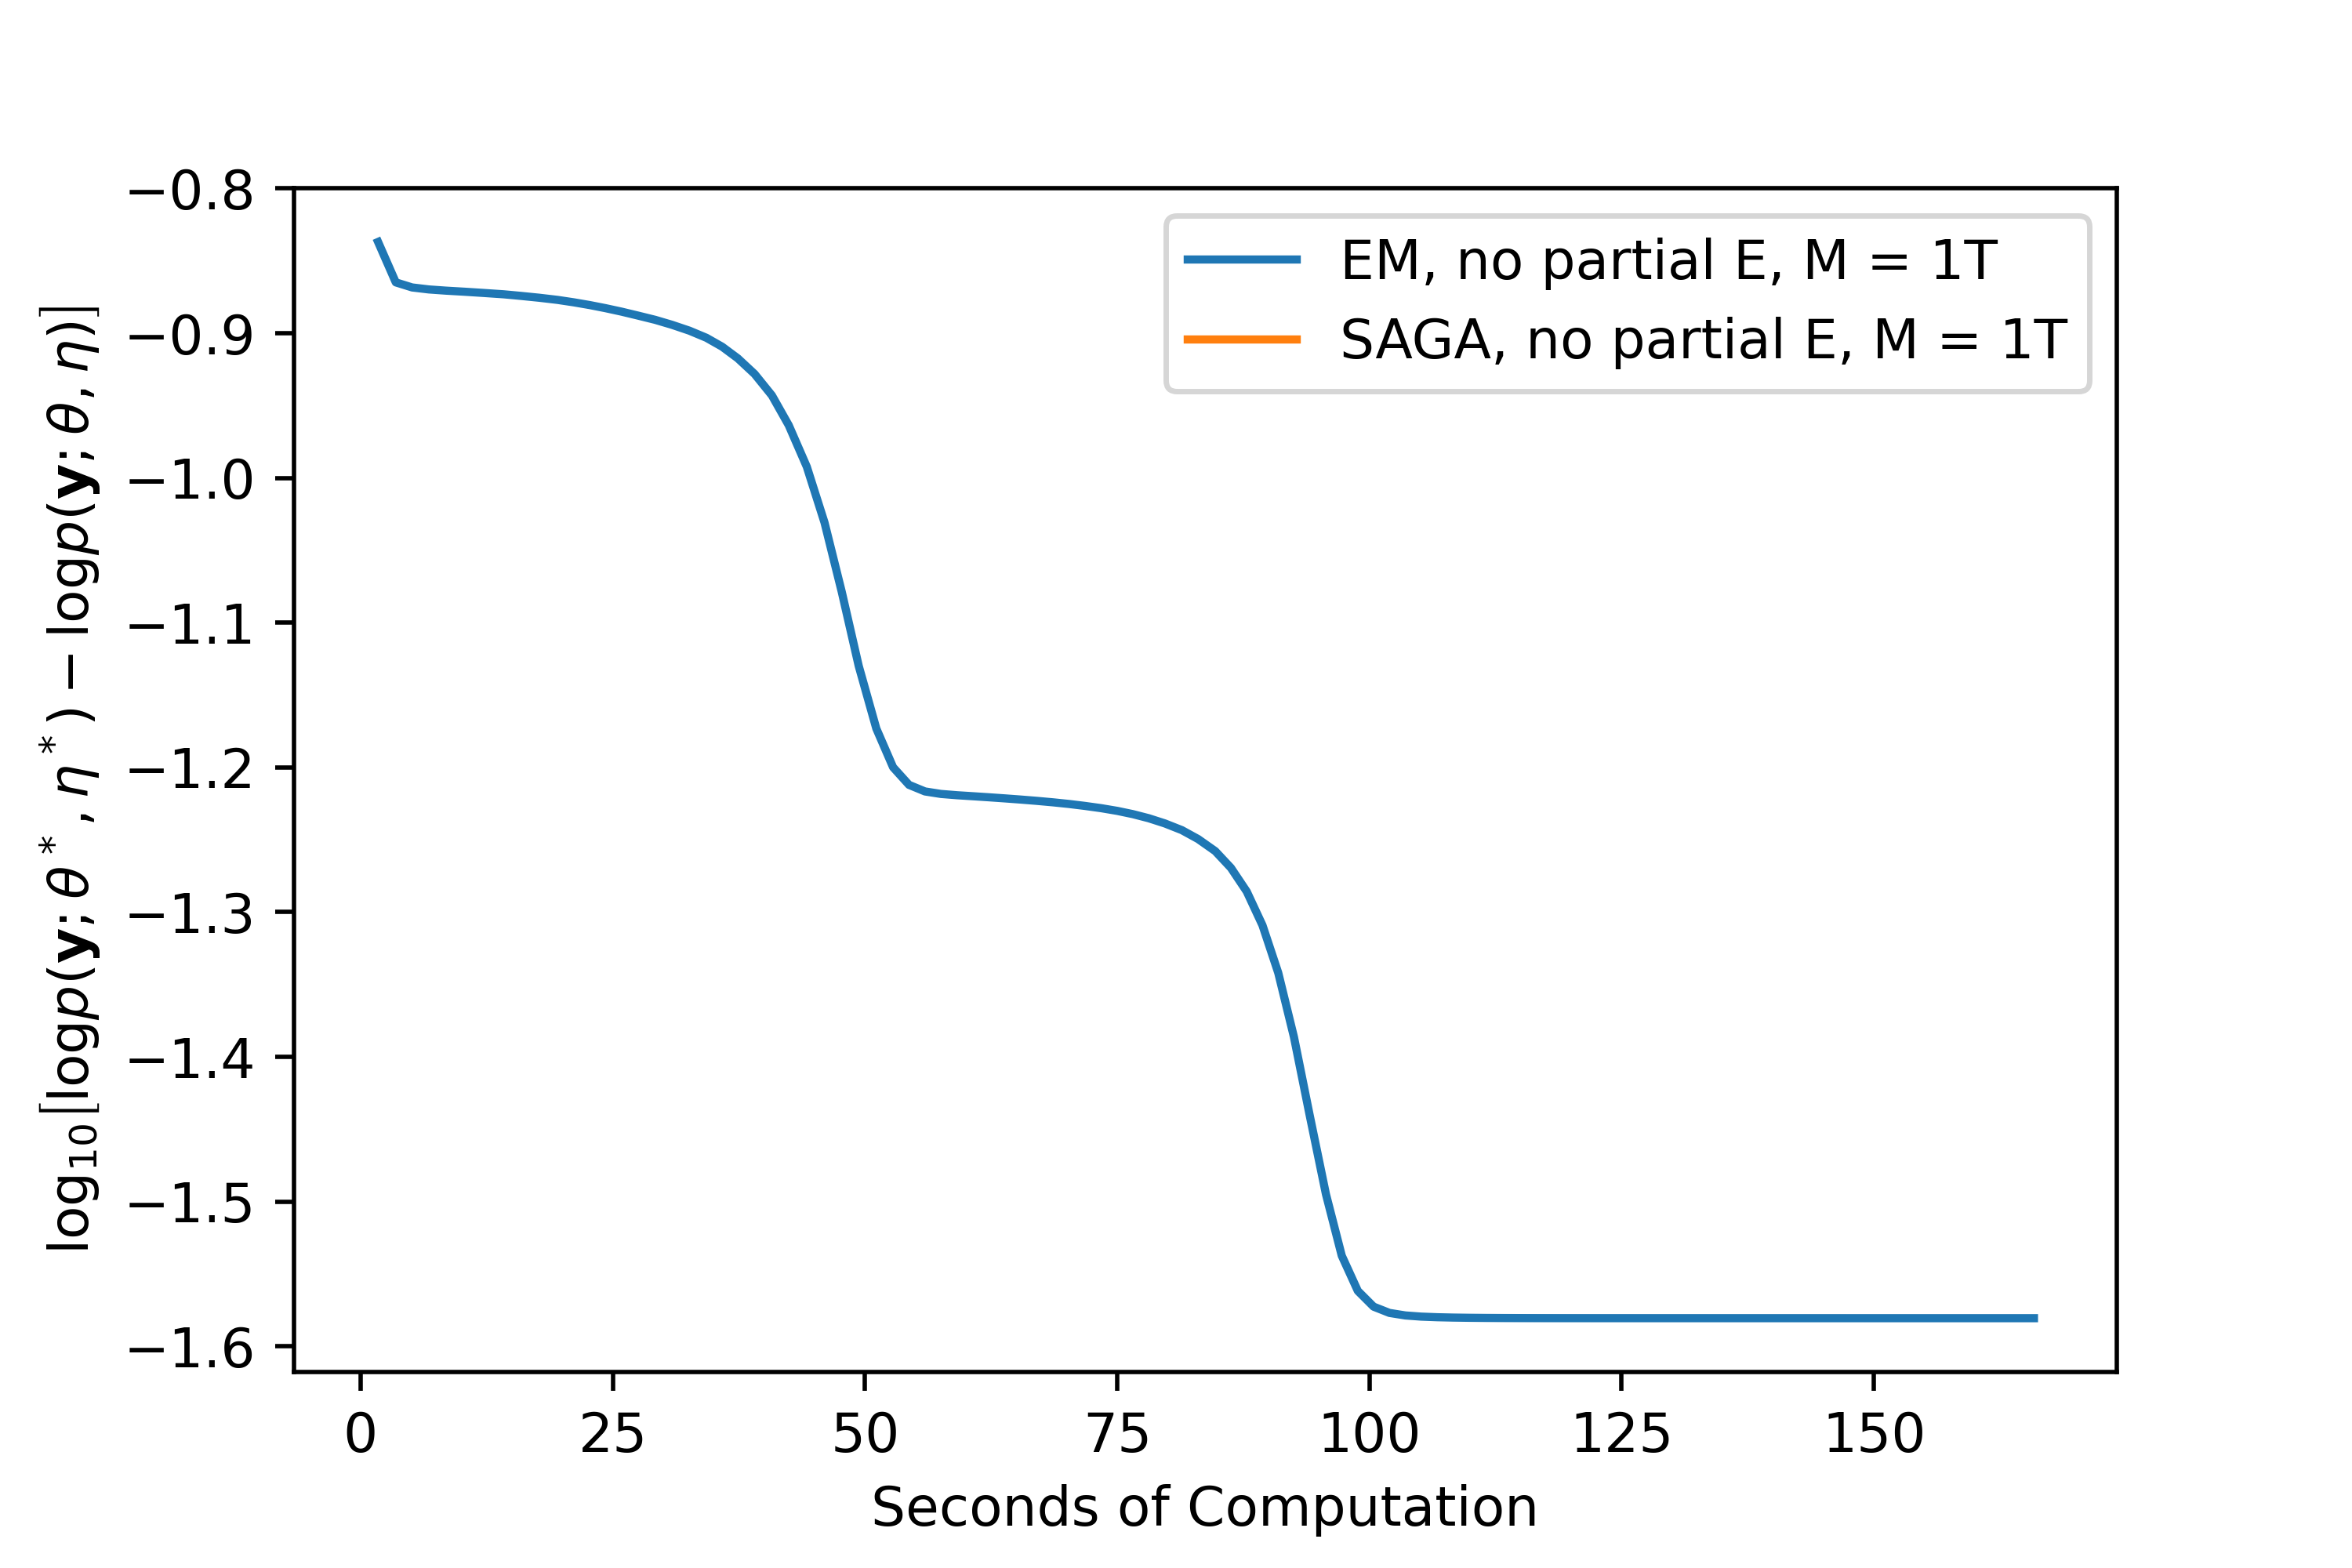
\includegraphics[width=3in]{../plt/log-like_v_time_exp_1.png}
    \caption{Optimally gap between the log-likelihood and optimal log-likelihood for the estimated parameters of the HMM from experiment 1 (rapid mixing). The figure on the left shows the optimality gap vs number of effective passes through the data set, while the figure on the right shows the optimality gap vs true computation time on a 2019 MacBook Pro. One epoch represents one full E-step, or one full M-step for variance reduced stochastic gradient methods. The y-axis is on a log-scale.}
    \label{fig:exp1_ll}
\end{figure}

\subsection{Experiment two: slow mixing}

The second experiment was to test the performance of the algorithm for a slowly mixing HMM. As such, we used the following transition probabilities:
%
\begin{equation*}
    \Gamma = 
    \begin{pmatrix} 
        0.99 & 0.005 & 0.005 \\
        0.005 & 0.99 & 0.005 \\
        0.005 & 0.005 & 0.99
    \end{pmatrix},
    \qquad
    \delta = \begin{pmatrix} 0.33 & 0.33 & 0.33 \end{pmatrix}
\end{equation*}
%
Figure (\ref{fig:exp2_ll}) displays the log-likelihood of the MLE parameters minus the log-likelihood at each epoch.
%
\begin{figure}
    \centering
    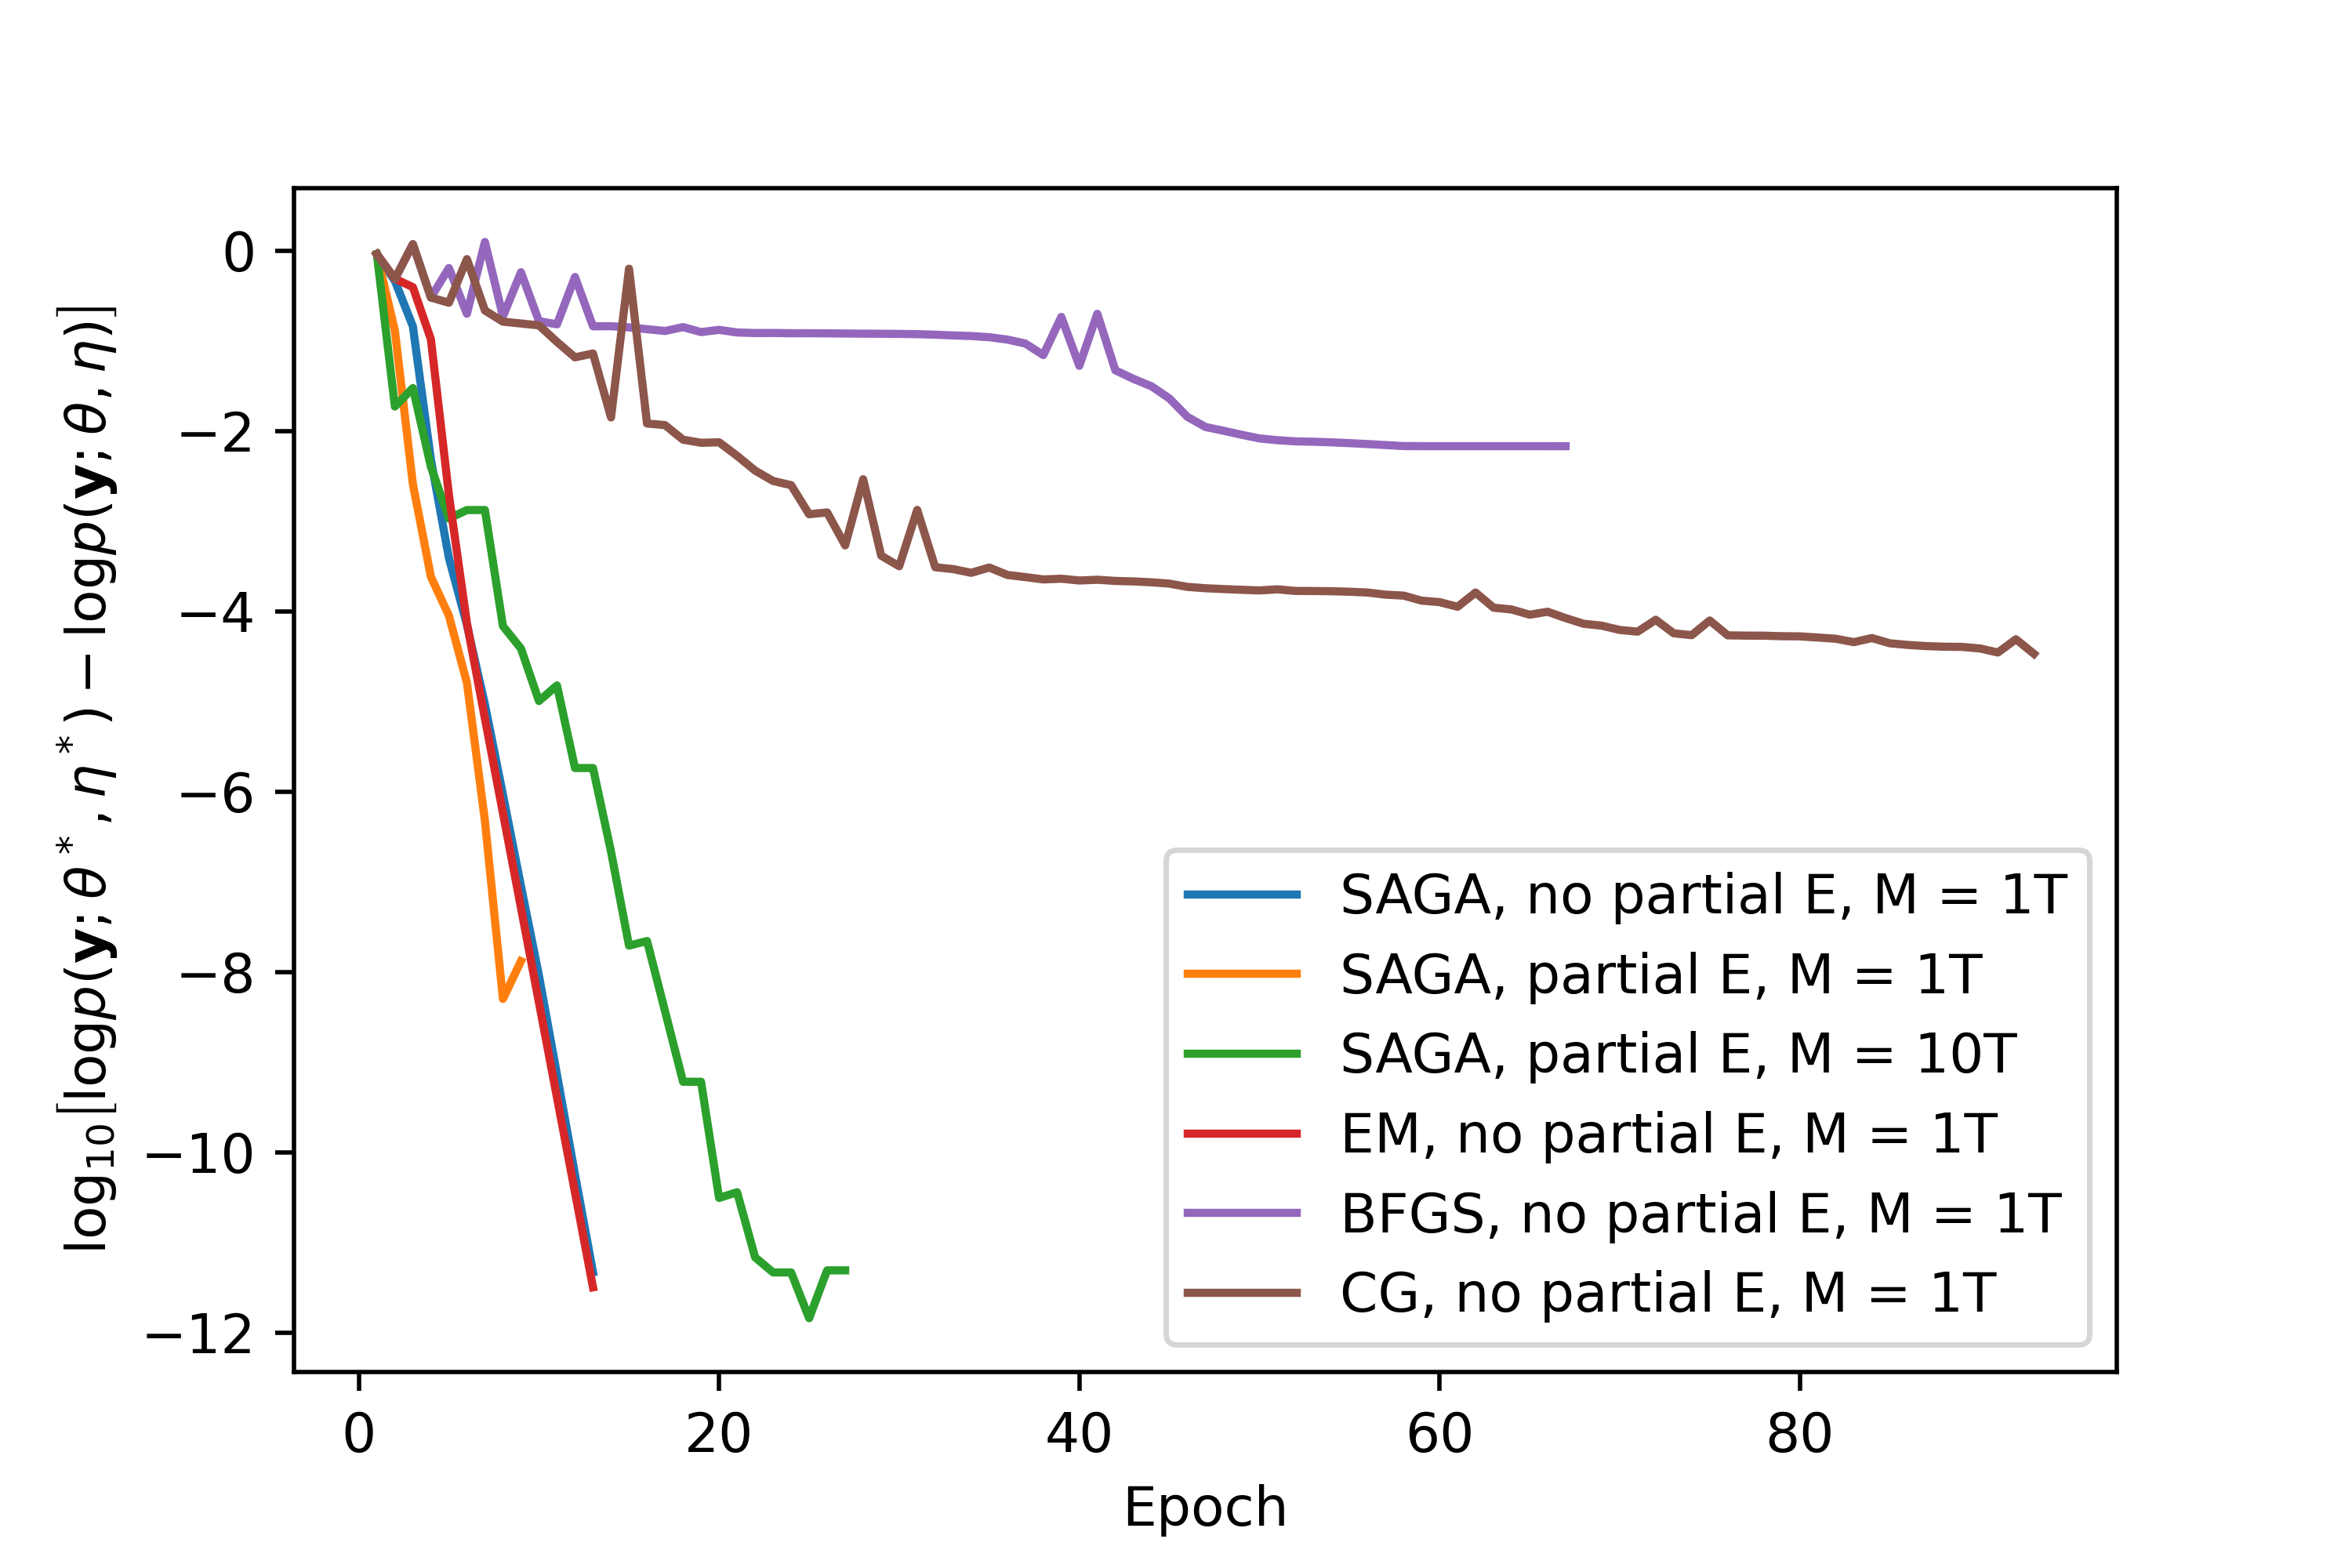
\includegraphics[width=3in]{../plt/log-like_v_epoch_exp_2.png}
    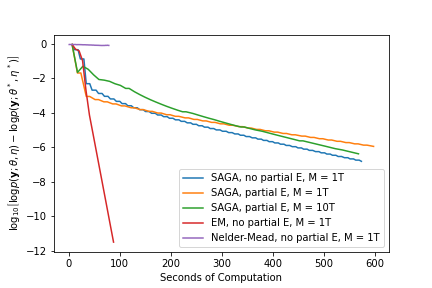
\includegraphics[width=3in]{../plt/log-like_v_time_exp_2.png}
    \caption{Optimally gap between the log-likelihood and optimal log-likelihood for the estimated parameters of the HMM from experiment 2 (slow mixing). The figure on the left shows the optimality gap vs number of effective passes through the data set, while the figure on the right shows the optimality gap vs true computation time on a 2019 MacBook Pro. One epoch represents one full E-step, or one full M-step for variance reduced stochastic gradient methods. The y-axis is on a log-scale.}
    \label{fig:exp2_ll}
\end{figure}